\documentclass[a4paper, 10pt, twoside, notitlepage]{article}
% idioma
\usepackage[spanish]{babel}
\usepackage[utf8x]{inputenc}
\usepackage{graphicx}

% graficos
%\usepackage[pdftex]{graphicx}
%\usepackage{wrapfig}

%\usepackage{listings}
%\lstset{language=C,basicstyle=\small}

%\usepackage{epic,eepic}
% estilo
\usepackage[footnotesize]{caption}
\usepackage[outer=2cm,inner=4cm,top=2cm,bottom=2cm]{geometry}
\usepackage{fancyhdr}
\usepackage{lipsum}
\usepackage{pdfpages}

\usepackage{color,hyperref}
\definecolor{black}{rgb}{0.0,0.0,0.0}
\definecolor{darkblue}{rgb}{0.0,0.0,0.3}

\hypersetup{colorlinks,breaklinks,
            linkcolor=black,urlcolor=darkblue,
            anchorcolor=darkblue,citecolor=darkblue}

% matematica
\usepackage{amsmath} \usepackage{amsfonts} \usepackage{amssymb}

\title{\textbf{Trabajo Práctico 1:\\Programación en MIPS} \\}

\author{ \\
         Ronnie Del Pino Cárdenas, \textit{Padrón 93575} \\
          \texttt{ delpinor@gmail.com }       \\
		  [2.5ex]
         Emiliano Vega, \textit{Padrón 76676}     \\
          \texttt{emiliano.vega@mail.com}                      \\
		  [2.5ex]
	 Romina Casal, \textit{Padrón 86429} \\
          \texttt{casal.romina@gmail.com}                      \\
		  [2.5ex]
		 \\
         \normalsize{2do. Cuatrimestre de 2019}            \\
         \normalsize{86.37 / 66.20 Organización de Computadoras $-$ Práctica Jueves} \\
         \normalsize{Facultad de Ingeniería, Universidad de Buenos Aires}
       }

\date{}

\begin{document}

\maketitle
% \thispagestyle{empty}   % quita el número en la primer página

% \newpage
% Es un breve resumen de lo que vamos a leer con mayor profundidad en las secciones posteriores, tiene que resaltar lo más importante.
\begin{abstract}
El presente trabajo práctico nos permitió realizar una comparativa entre la performance de dos implementaciones de un programa en C basado en el algoritmo "La hormiga artista" del trabajo práctico anterior en varios niveles de optimización y reemplazando dos funciones clave a código MIPS. Para el análisis se utilizó el programa /usr/bin/time que nos da los tiempos de ejecución resultante.
\end{abstract}

% \tableofcontents
%
% \newpage
%

\pagestyle{fancy}
\fancyhead{}
\fancyfoot{}
\renewcommand{\sectionmark}[1]{\markright{\thesection\ #1}}
\renewcommand{\headrulewidth}{0.4pt}
%\renewcommand{\footrulewidth}{0.4pt}
\fancyhead[LE]{\nouppercase \rightmark}
\fancyhead[RE, LO]{\bf \thepage}
\fancyhead[RO]{\nouppercase \rightmark}
\fancyfoot[C]{ }
\maketitle
%genera el indice - compilar dos veces
\setcounter{page}{1}
% \tableofcontents
% \newpage

\parskip 7.2pt
%Distinto al resumen, se dice cual es el objetivo principal y se hace un resumen de cada parte que aparece a continuación.
\section{Introducción}
Para la realización de las pruebas se ha creado un Makefile adaptado que permite compilar las versiones tp1\_if y tp1\_tables en los niveles 0, 1, 2 y 3 de optimización que ofrece gcc, además de las versiones con las funciones new\_orientation y move\_forward en código assembly.\\
Se realizará la ejecución de varias opciones de iteraciones con estas versiones para comparar los distintos tiempos de ejecución y observar la tasa de mejora lograda.\\

%Una de las secciones más importantes del informe. Aquí se explaya todo lo realizado, problemas encontrados y soluciones propuestas con variantes y métricas.

\newpage

\section{Proceso de Compilación}

Se adaptó el archivo makefile provisto por la cátedra para generar los ejecutables con las distintas opcioens de optimización para el código integralmente en C.\\

\begin{itemize}
\item[] \textbf{make all\_tp1\_c}: Crea los ejecutables tp1\_if\_opt0, tp1\_if\_opt1, tp1\_if\_opt2, tp1\_if\_opt3 para la versión con jumps en los distintos niveles de optimización, y tp1\_tables\_opt0, tp1\_tables\_opt1, tp1\_tables\_opt2, tp1\_tables\_opt3 para la versión con table.
\item[] \textbf{make tp1\_tables\_asm}: Crea el ejecutable tp1\_tables\_asm para la versión con table que tiene las funciones new\_orientation y move\_forward en assembly.
\item[] \textbf{make tp1\_if\_asm}: Crea el ejecutable tp1\_if\_asm para la versión con jumps que tiene las funciones new\_orientation y move\_forward en assembly.
\end{itemize}

Creamos un archivo script pruebas.sh que usando \textbf{/usr/bin/time} cuenta el tiempo de ejecución de cada prueba y guarda los resultados en un archivo \textbf{test\_result.txt}
Con los valores obtenidos en este archivo se crearon gráficas comparativas de tiempo de ejecución en función de la cantidad de iteraciones.\\

Por ejemplo, la línea:

\scriptsize
\begin{verbatim}
/usr/bin/time --output=test_result.txt -a -f "%E\treal\t%U\tuser\t%S\tsys" ./tp1_if_opt0 -g 1000x1000 -p RGBW -r LLLL -t $((10000)) > /dev/null
\end{verbatim}
\normalsize

Escribirá el siguiente resultado en \textbf{test\_result.txt}:
\scriptsize
\begin{verbatim}
0:11.39	real	11.14	user	0.03	sys
\end{verbatim}
\normalsize

De esa medición usaremos el tiempo real de ejecución obtenido para las comparaciones.\\
NOTA: Es probable que sea necesario instalar en la VM ejecutada con QEMU el programa time que tiene opciones adicionales que el homónimo que trae por defecto no permite usar.\\

\newpage
\section{Desarrollo}
<<ACA ESCRIBIMOS SOBRE LAS DECISIONES DE DESARROLLO>> \\
\\

Ejecutamos el script \textbf{pruebas.sh} y arroja los siguientes resultados que exporta al archivo \textbf{test_result.txt}
<< FALTAN LAS PRUEBAS DE ASM >>
\scriptsize
\begin{verbatim}
Pruebas TP1
Grafico de iteraciones
tp1_if - optimizacion 0
0:11.39	real	11.14	user	0.03	sys
0:12.41	real	12.35	user	0.04	sys
0:12.19	real	12.16	user	0.02	sys
0:18.53	real	18.50	user	0.01	sys
1:19.81	real	79.50	user	0.04	sys
11:41.06	real	700.63	user	0.03	sys
tp1_if - optimizacion 1
0:10.25	real	10.20	user	0.03	sys
0:10.66	real	10.62	user	0.02	sys
0:10.18	real	10.14	user	0.03	sys
0:15.36	real	15.30	user	0.04	sys
0:50.10	real	50.03	user	0.02	sys
6:47.14	real	406.88	user	0.02	sys
tp1_if - optimizacion 2
0:11.16	real	11.12	user	0.03	sys
0:11.11	real	11.08	user	0.02	sys
0:12.02	real	11.96	user	0.04	sys
0:18.66	real	18.62	user	0.02	sys
0:47.17	real	47.12	user	0.02	sys
6:26.73	real	386.48	user	0.03	sys
tp1_if - optimizacion 3
0:09.87	real	9.83	user	0.02	sys
0:09.99	real	9.95	user	0.02	sys
0:11.56	real	11.52	user	0.02	sys
0:14.15	real	14.12	user	0.01	sys
0:45.25	real	45.21	user	0.00	sys
6:00.04	real	359.80	user	0.03	sys
tp1_tables - optimizacion 0
0:09.61	real	9.57	user	0.01	sys
0:11.39	real	11.37	user	0.00	sys
0:12.67	real	12.63	user	0.02	sys
0:22.76	real	22.71	user	0.03	sys
1:47.64	real	107.54	user	0.03	sys
17:00.54	real	1019.67	user	0.05	sys
tp1_tables - optimizacion 1
0:08.93	real	8.89	user	0.02	sys
0:10.60	real	10.56	user	0.02	sys
0:12.15	real	12.11	user	0.02	sys
0:14.79	real	14.74	user	0.03	sys
0:55.26	real	55.21	user	0.01	sys
8:04.03	real	483.73	user	0.02	sys
tp1_tables - optimizacion 2
0:11.35	real	11.31	user	0.02	sys
0:10.24	real	10.19	user	0.04	sys
0:12.67	real	12.61	user	0.03	sys
0:16.59	real	16.55	user	0.02	sys
0:59.45	real	59.38	user	0.03	sys
10:28.80	real	628.41	user	0.04	sys
tp1_tables - optimizacion 3
0:09.76	real	9.71	user	0.03	sys
0:11.14	real	11.10	user	0.02	sys
0:10.42	real	10.37	user	0.03	sys
0:17.49	real	17.45	user	0.02	sys
0:59.53	real	59.45	user	0.03	sys
8:16.94	real	496.64	user	0.02	sys
\end{verbatim}
\normalsize

<< CONCLUSIONES SOBRE LOS RESULTADOS Y GRAFICOS >>
\\
\\

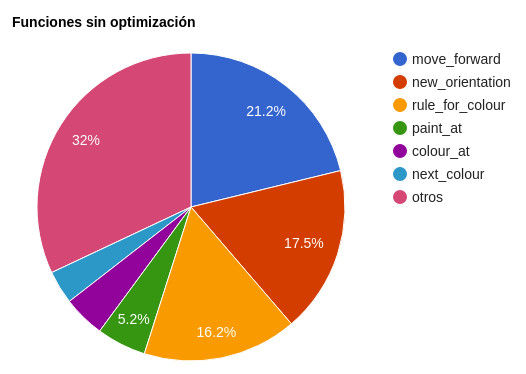
\includegraphics[scale=3]{chart.jpg} \\

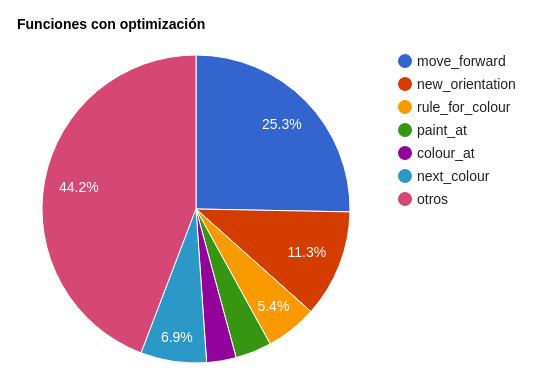
\includegraphics[scale=3]{chart2.jpg} \\

\newpage

\section{Conclusión}
<< CONCLUSIONES FINAL >>


\vspace{.5cm}
%Referencias o recursos utilizados durante la investigación para la resolución del trabajo práctico
\begin{thebibliography}{5}
 \bibitem{} La Universidad de Pensilvania.\\ \url{http://www.cse.psu.edu/~pdm12/cmpsc311-f16/}.
 \bibitem{} Profiling and Timing Code
.\\ \url{https://jakevdp.github.io/PythonDataScienceHandbook/01.07-timing-and-profiling.html}.
 \bibitem{} C to MIPS compiler
.\\ \url{http://reliant.colab.duke.edu/c2mips/}.
\end{thebibliography}

\clearpage

\part{Apéndice}
\appendix

\section{Enunciado original}\label{sec:enunciado}
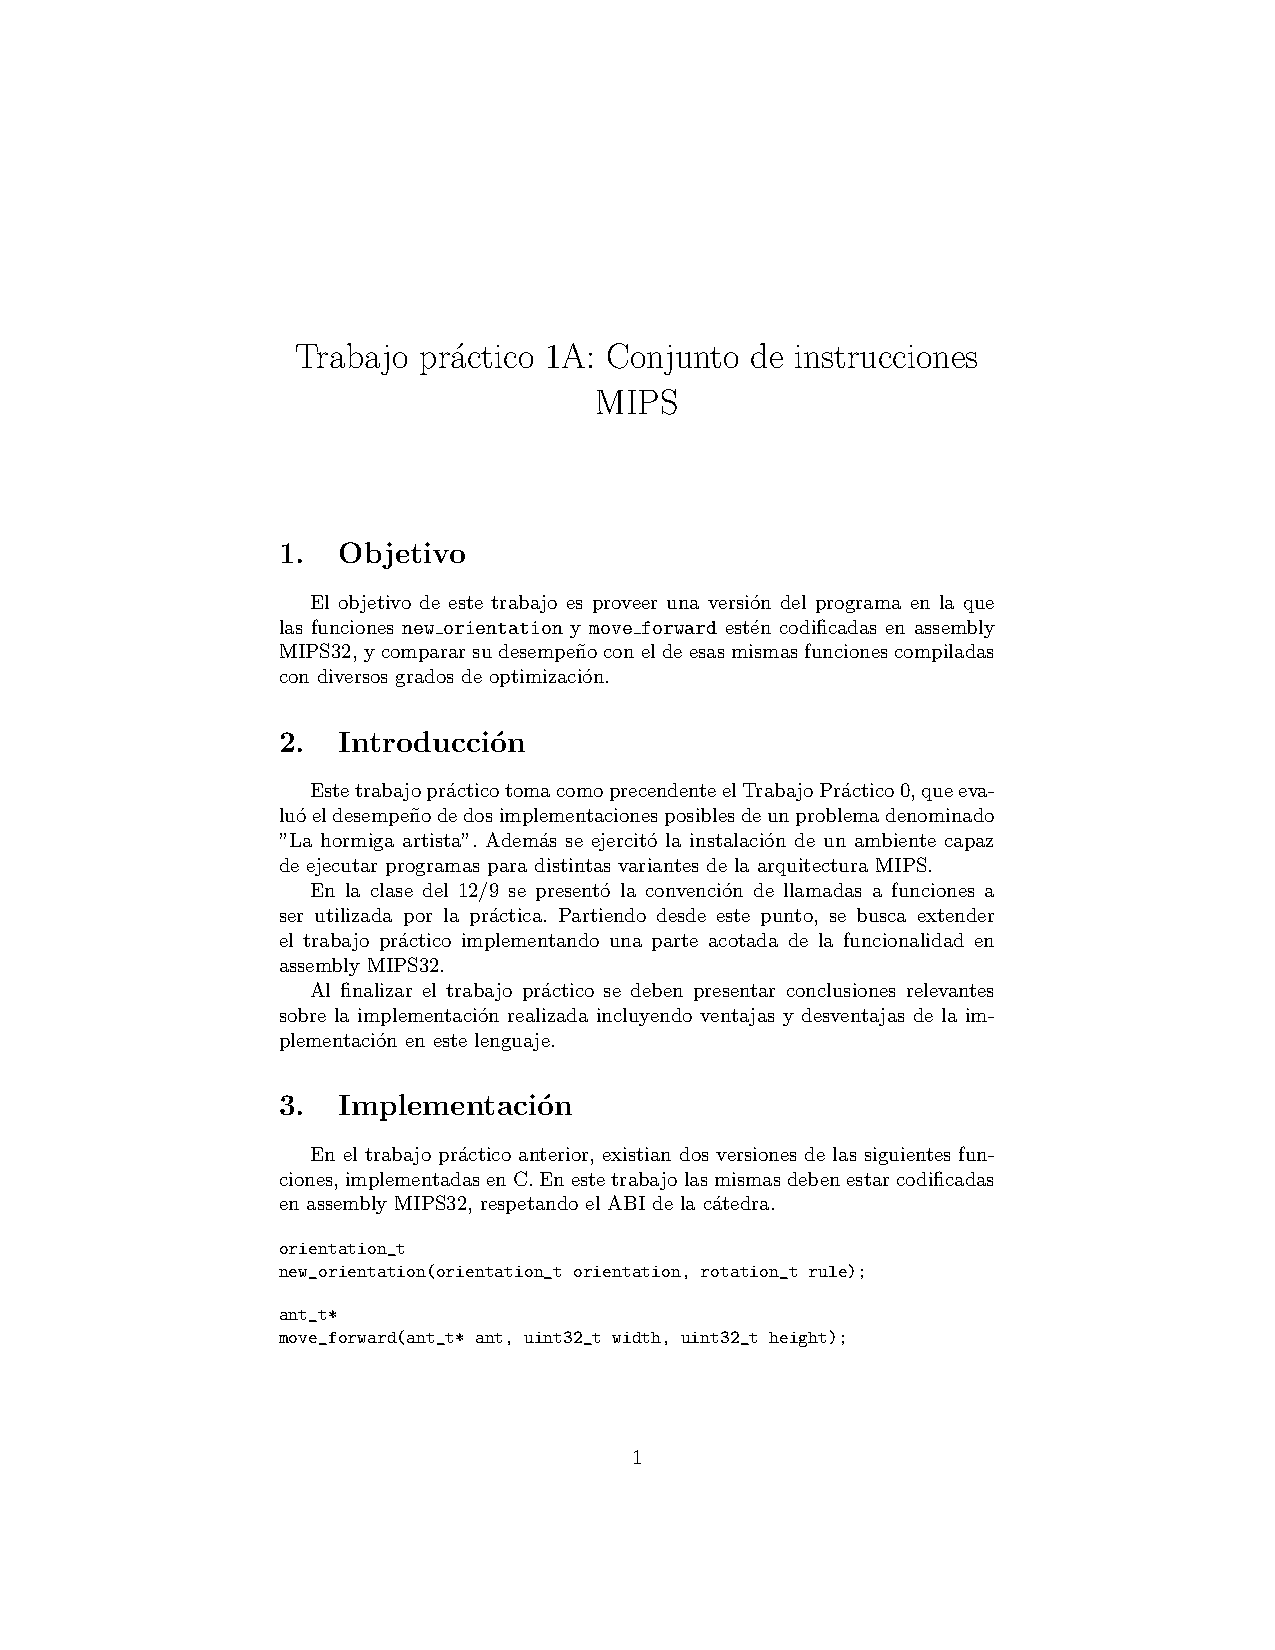
\includepdf[pages={-}]{enunciado.pdf}

\end{document}
